\chapter*{Mathematical Synthesis}
\addcontentsline{toc}{chapter}{Mathematical Synthesis}

Machine Intelligence II begins from unsupervised structure: what can be learned when the data arrive without labels? Principal component analysis is the clean prototype because every step is visible. Center the data, measure covariance, diagonalize the covariance, project onto the strongest directions, and track exactly what variance was kept or discarded.

\begin{figure}[h]
\centering
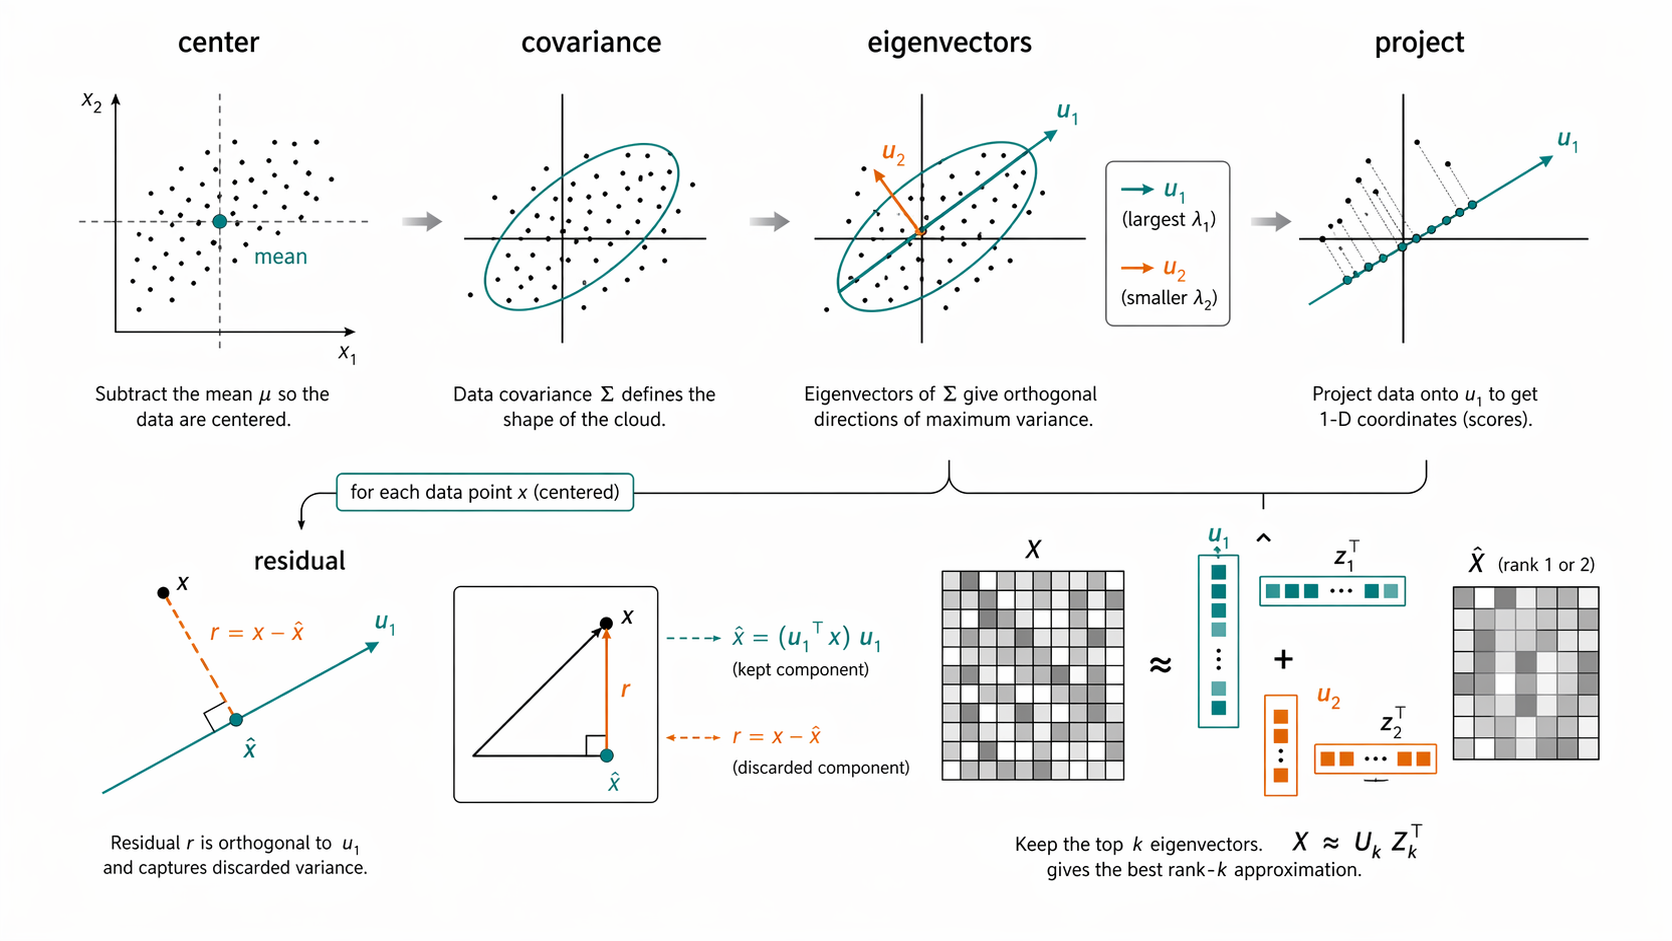
\includegraphics[width=0.96\textwidth]{figures/codex-mi2-pca-spectral-compression.png}
\caption{PCA as spectral compression. Centering removes the mean, the covariance ellipse reveals directions of variation, eigenvectors provide orthogonal coordinates, projection keeps high-variance coordinates, and residuals are the discarded orthogonal variation.}
\end{figure}

\section*{The Covariance Matrix Is A Geometry}

Let centered data vectors be rows of \(X\in\R^{n\times d}\). The empirical covariance is
\[
  \Sigma
  =
  \frac{1}{n}X^\top X.
\]
For any unit direction \(u\), the variance of the data after projection onto \(u\) is
\[
  \frac{1}{n}\|Xu\|^2
  =
  u^\top \Sigma u.
\]
So PCA asks for the direction with maximal quadratic form:
\[
  u_1
  \in
  \operatorname*{arg\,max}_{\|u\|=1} u^\top \Sigma u.
\]
The solution is the leading eigenvector of \(\Sigma\). The corresponding eigenvalue is the variance captured along that direction.

\section*{Projection And Reconstruction}

If \(U_k=[u_1,\dots,u_k]\) contains the top \(k\) orthonormal eigenvectors, then the low-dimensional score vector for a data point \(x\) is
\[
  z = U_k^\top x,
\]
and the rank-\(k\) reconstruction is
\[
  \hat{x} = U_k z = U_kU_k^\top x.
\]
The residual is
\[
  r = x-\hat{x}.
\]
It is orthogonal to the retained subspace, so the reconstruction separates data into an explained component and a discarded component.

\begin{keyequation}[Variance captured]
\[
  \text{captured variance}(k)
  =
  \sum_{j=1}^{k}\lambda_j,
  \qquad
  \text{fraction captured}
  =
  \frac{\sum_{j=1}^{k}\lambda_j}{\sum_{j=1}^{d}\lambda_j}.
\]
\tcblower
The spectrum \(\lambda_1\ge \lambda_2\ge \cdots\ge \lambda_d\) is a diagnostic for intrinsic dimension. A fast spectral decay means the data are close to a low-dimensional subspace.
\end{keyequation}

\section*{Why PCA Is The Right Baseline}

PCA is linear, unsupervised, and global. Those limitations are also why it is such a useful baseline. If a nonlinear representation method improves on PCA, it should be clear which PCA assumption it breaks: linearity, globality, Euclidean reconstruction error, or Gaussian-like covariance structure.

The mathematical virtue of PCA is that it solves two problems at once. It maximizes retained variance and minimizes squared reconstruction error:
\[
  \min_{\mathrm{rank}(\hat{X})\le k}
  \|X-\hat{X}\|_F^2.
\]
By the Eckart--Young theorem, the solution is the truncated singular value decomposition. This makes PCA the reference point for later factor models, autoencoders, manifold learning, and probabilistic latent-variable models.
